\subsection{Vertex+Beamspot Constraint: VXBS}
Leptons produced from the \hzzfourl channel should originate from the \pp collision point---the primary vertex---since the \PH boson and both \PZ bosons decay promptly after being formed.
The primary vertex from which the muons originate can be approximated to come from the more general \emph{beamspot}, \ie the luminous region in the $x$-$y$ plane where the \pp bunches cross.
Thus, if the muon tracks are constrained to come from their vertex of origination ($\sim$beamspot), then one should expect a more precise measurement of muon momentum and resolution.
The updated muon kinematical variables then get propagated into a more precise estimate of the \mH value per event.
This process of constraining muon tracks to a vertex that is compatible with the beamspot is called the `vertex+beamspot constraint' (VXBS).

The Phase-1 pixel upgrade during the middle of Run 2 allowed for a more collimated (\emph{more precise}) \pp beamspot.
\Cref{fig:BeamY_vs_Y} shows the improvement on a tighter beamspot when moving from 2016 Run G to 2018 Run D.
Both the $x$ and $y$ widths of the beamspot ($\sigma_x$ and $\sigma_y$, respectively) are smaller:
\begin{align*}
    \sigma_x^{2016} \sim 14\mum \quad &  \vs \quad \sigma_x^{2018} \sim 9\mum
    \\
    \vspace{3pt}
    \sigma_y^{2016} \sim 9\mum \quad &  \vs \quad \sigma_y^{2018} \sim 7\mum,
\end{align*}
giving a better vertex constraint for muons when it is used in the track reconstruction.
Once the event is selected, the vertex+beamspot constraint is applied.
%%%%%%%%%%%%%%%%%%%%%%%%%%%%%%%
% Beamspot width Y \vs. width X.
\begin{multiFigure}
    \centering
        \addFigure{0.48}{figures/higgsmassmeas/vxbs/2016G_VS_width_y_vs_x_workinprogress.png}
        \addFigure{0.48}{figures/higgsmassmeas/vxbs/2018D_VS_width_y_vs_x_workinprogress.png}
	\captionof{figure}
        [Two-dimensional histogram of beamspot widths, $\sigma_y$ \vs $\sigma_x$, comparing 2016 Run G and 2018 Run D]
        {Two-dimensional histogram of beamspot widths (in \cmns), $\sigma_y$ \vs $\sigma_x$ for different runs.
        The 2018 runs showed narrower beamspot spreads, which assists with the vertex+beamspot constraint.
        \;A) For 2016 Run G.
        \;B) For 2018 Run D.}
    \label{fig:BeamY_vs_Y}
\end{multiFigure}
%%%%%%%%%%%%%%%%%%%%%%%%%%%%%%%

The muon reconstruction that is currently used does not take into account any information about the vertex from which the lepton originates. % and in the Higgs boson decay, all the leptons are prompt.
In the VXBS approach, the four muon tracks from a Higgs boson decay are constrained to a common vertex (VX) that must be compatible with the beamspot (BS). 
So while the kinematical information of muons is updated after this procedure, the information of electrons is left unaltered, as they are only used to help constrain the position of the common vertex.

This method has been checked in data and simulation using \ztomumu events, looking in the \mZ range of 60--120\GeV.
The improvement of muon momentum resolution is shown in \cref{fig:Resolution_pT,fig:Resolution_eta}, as a function of \pT and $|\eta|$, respectively, for 2016--2018.
It was seen that \pT resolution and \mZ resolution improves by about 5--10\%, depending on the year.
\begin{multiFigure}
    \centering
        \addFigure{0.48}{figures/higgsmassmeas/vxbs/Resolution_2016_preVFP_PT_workinprogress.png}
        \addFigure{0.48}{figures/higgsmassmeas/vxbs/Resolution_2016_postVFP_PT_workinprogress.png}
        \addFigure{0.48}{figures/higgsmassmeas/vxbs/Resolution_2017_PT_workinprogress.png}
        \addFigure{0.48}{figures/higgsmassmeas/vxbs/Resolution_2018_PT_workinprogress.png}
    \captionof{figure}
        [Muon \pT resolution as a function of \pT before and after VXBS constraint]
        {Muon \pT resolution as a function of \pT before (black line) and after (red line) VXBS constraint using \ztomumu events in data.
        The ratio plot at the bottom of each subfigure shows improvement in muon \pT resolution, with improvement as high as approximately 15\% in 2018 events.
        \;A) For 2016 pre-VFP.
        \;B) For 2016 post-VFP.
        \;C) For 2017.
        \;D) For 2018.}
    \label{fig:Resolution_pT}
\end{multiFigure}
\begin{multiFigure}
    \centering
        \addFigure{0.48}{figures/higgsmassmeas/vxbs/Resolution_2016_preVFP_ETA_workinprogress.png}
        \addFigure{0.48}{figures/higgsmassmeas/vxbs/Resolution_2016_postVFP_ETA_workinprogress.png}
        \addFigure{0.48}{figures/higgsmassmeas/vxbs/Resolution_2017_ETA_workinprogress.png}
        \addFigure{0.48}{figures/higgsmassmeas/vxbs/Resolution_2018_ETA_workinprogress.png}
    \captionof{figure}
        [Muon \pT resolution as a function of \abseta before and after VXBS constraint]
        {Muon \pT resolution as a function of \abseta before (black line) and after (red line) VXBS constraint using \ztomumu events in data.
        The ratio plot at the bottom of each subfigure shows improvement in muon \pT resolution, with improvement as high as approximately 10\% for all years.
        \;A) For 2016 pre-VFP.
        \;B) For 2016 post-VFP.
        \;C) For 2017.
        \;D) For 2018.}
\label{fig:Resolution_eta}
\end{multiFigure}

\Cref{UL_ZBoson_DataMC_comparison_VXBS} shows Data--MC comparison, with and without VXBS constraint.
The mean and $\sigma$ reported on the plots belong to the DSCB---which is convolved with a BW---and fit to the distribution.
As can been seen, the resolution of \mll gets improved comparably to that of the improvement of muon \pT resolution:
5\% (5\%) for 2016 pre-VFP,
5\% (6\%) for post-VFP,
5\% (4\%) for 2017, and
7\% (8\%) for 2018 Data (MC).
\begin{multiFigure}
    \centering
        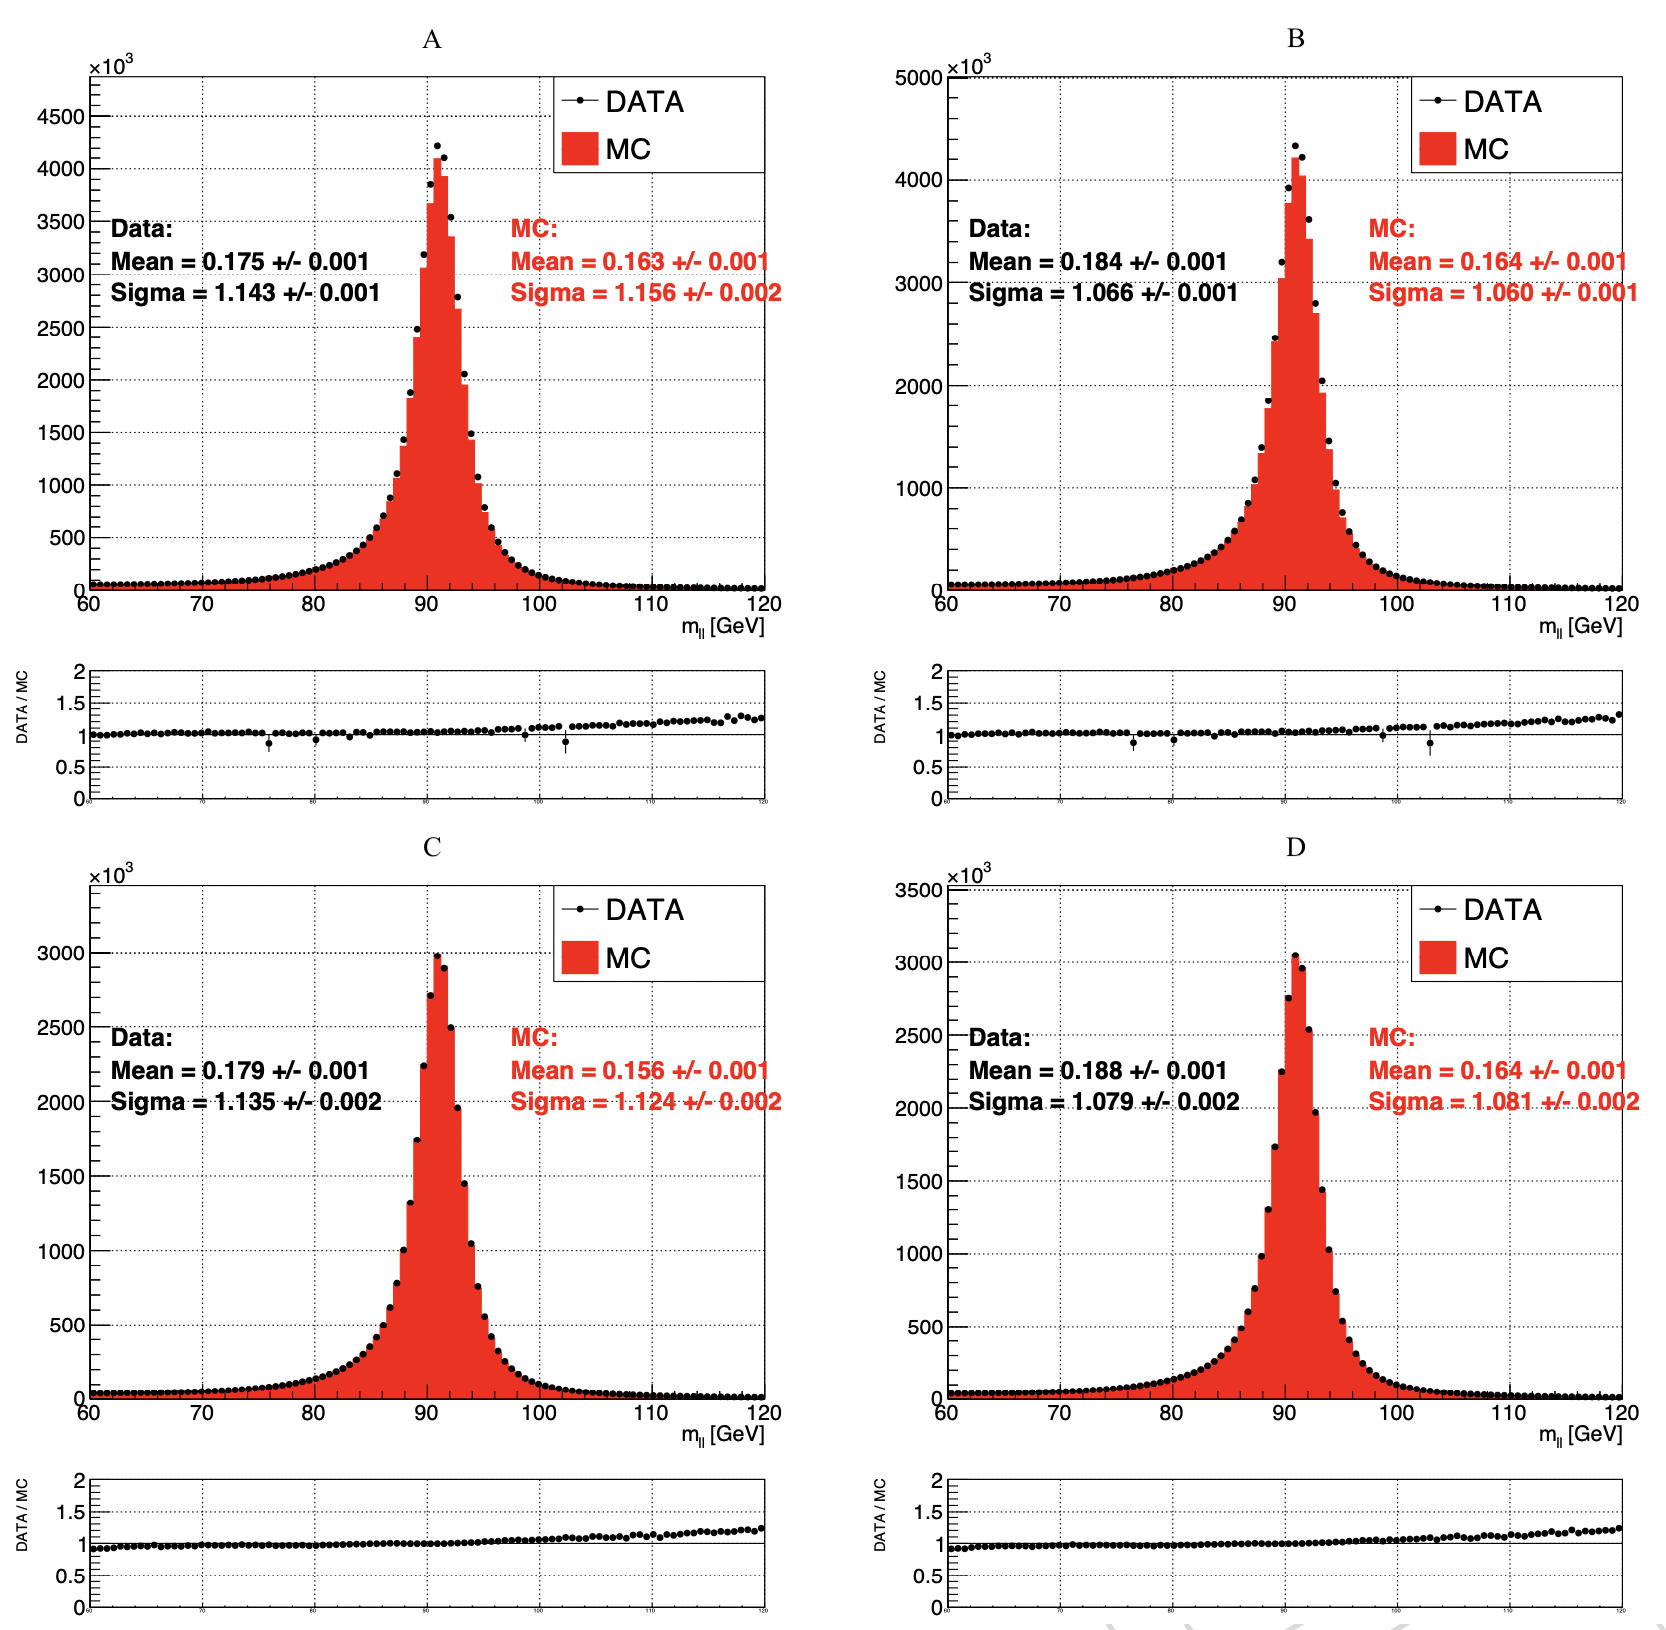
\includegraphics[width=0.96\textwidth]{figures/higgsmassmeas/vxbs/vxbs_mZdist_2017_2018.png}
    \captionof{figure}
        [Distributions of \mll using data and MC, with and without the VXBS constraint]
        {Distributions of \mll using data and MC, with (left column) and without (right column) the VXBS constraint. % TODO: REWORD 
        \;A) 2018.
        \;B) 2017.
        \;C) 2016 post-VFP.
        \;D) 2016 pre-VFP.}
    \label{UL_ZBoson_DataMC_comparison_VXBS}
\end{multiFigure}

%=== 1D likelihood fit after VXBS ===%
The updated invariant mass distributions, after applying the VXBS constraint, are shown in Fig.~\ref{fig:1D_VXBS_mass_2018_ggH}.
\begin{multiFigure}
    \centering
        \addFigure{0.45}{figures/higgsmassmeas/ggH_MassDistribution/1D_VXBS_mass_2018_ggH_4mu.pdf}
        \addFigure{0.45}{figures/higgsmassmeas/ggH_MassDistribution/1D_VXBS_mass_2018_ggH_4e.pdf}
        \addFigure{0.45}{figures/higgsmassmeas/ggH_MassDistribution/1D_VXBS_mass_2018_ggH_2e2mu.pdf}
        \addFigure{0.45}{figures/higgsmassmeas/ggH_MassDistribution/1D_VXBS_mass_2018_ggH_2mu2e.pdf}
    \captionof{figure}
        [Four-lepton invariant mass distribution, after applying the VXBS constraint]
        {Four-lepton invariant mass distribution, after applying the VXBS constraint in the signal region ([105-140]\GeV) using ggH events, with the DSCB fit for 2018.
        \;A) \fourmu.    % TODO: fix symbols
        \;B) \foure.
        \;B) \twoetwomu.
        \;B) \twomutwoe.}
    \label{fig:1D_VXBS_mass_2018_ggH}
\end{multiFigure}
As can been seen, comparing these new distributions (\cref{fig:1D_VXBS_mass_2018_ggH}) with the ones before beamspot constraint (\cref{fig:1D_VXBS_mass_2018_ggH}), the $\sigma$ in \fourmu final state has improved by 7$\%$, \foure is not affected (as expected), while mixed flavor final states show an improvement of a few percent.

\subsubsection{Expected \mH measurement uncertainties (MC)}
The expected $\mass{\PH}$ measurement uncertainties comparing VXBS constraint to the baseline expectations can be seen in \cref{table:1D_model_result_fs_BS} split by final state or in \cref{table:1D_model_result_year_BS} split by year.

\begin{table}[ht]	
\begin{center}
    \captionof{table}
        [Expected Higgs boson mass uncertainty measured with 1D model, with and without VXBS, by final state]
        {Expected Higgs boson mass uncertainty measured with 1D model, with and without
        VXBS for different final states. All mass values are given in \MeVns.
        Statistical-only results are considered at this stage of the analysis.}
    \begin{tabular}{ccccccc}
            \hline			
        Expected uncertainty (\MeVns)	&	\fourmu	&	\foure	&	\twoetwomu	&\twomutwoe	& inclusive	& Rel. Improvement \\
            \hline			
        1$D_\text{VXBS}$  (No bkg)	&	137	&	394	&	275	&	266	&	108 &	$-$4\%	\\
            1D	(No bkg) &	147	&	394	&	276	&	273	&	112	&	---	\\
        %	1$D_\text{VXBS}$  (No bkg)	&	144	&	466	&	313	&	291	&	116	&	-4\%	\\	
        %	1D	(No bkg) &	153	&	466	&	315	&	300	&	121 	&	- \\
            \hline
    \end{tabular}
    \label{table:1D_model_result_fs_BS}
\end{center}
\end{table}
\begin{table}[ht]	
\begin{center}
    \captionof{table}
        [Expected Higgs boson mass uncertainty measured with 1D model, with and without VXBS, by year]
        {Expected Higgs boson mass uncertainty measured with 1D model, with and without VXBS for different years. All mass values are given in \MeVns.
        Statistical-only results are considered at this stage of the analysis.}
    \begin{tabular}{ccccc}
        \hline			
    Expected uncertainty (\MeVns)	&	2016 pre-VFP	&	2016 post-VFP	&	2017	&	2018	\\
        \hline			
        1$D_\text{VXBS}$	(No bkg)	&	291	&	301	&	198	&	162	\\
        1D (No bkg)	&	304	&	314	&	207	&	170	\\
        \hline
    \end{tabular}
    \label{table:1D_model_result_year_BS}
\end{center}
\end{table}

\subsubsection{Alternative to VXBS: The Ad Hoc Method}
It was seen that the lepton \pT resolution depends upon the product of lepton charge $(q)$ and lepton impact parameter $(d_0)$.
See Appendix~\ref{app:adhoc_studies} for a motivation of this study and derivation of the formula for $d_0$.
